\documentclass{article}
\usepackage{amsmath, amssymb}
\usepackage{graphicx}
\usepackage{titlesec}
\usepackage[font=small,labelfont=bf]{caption} % Required for specifying captions to tables and figures
\usepackage[margin=1in,footskip=0.2in]{geometry}

\title {\vspace{-5em}Computer Vision}
\author{\vspace{-8em}nkgp46}
\date{\vspace{-1em}December 3, 2019}

\titlespacing*{\section}
{0pt}{0ex plus 0ex minus -2ex}{0.3ex plus .2ex}

\setlength{\parindent}{0em}
\setlength{\parskip}{1em}


\begin{document}
	\maketitle
	
	\section{Object detection}
	
	YOLO was used for object detection. Out of 34 selected test frames, without any pre-processing, it detected a total of 318 objects of which 4 objects were erroneous, giving an accuracy of 98.74\% on the test set. On some frames the algorithm failed to detect objects, however this mostly occurred on objects that were far away, occluded or distorted due to lighting or noise. Increasing the confidence threshold of YOLO from 0.5 to 0.55 reduced the total number of detected objects by 10. To improve the performance of the implementation practically, a GPU enabled YOLO implementation should be used, as this would reduce the average object detection speed of $\approx 1.22s$ by a large amount.
	
	\section{Comparison of disparity calculation techniques}
	
	Monocular, pyramid stereo matching and OpenCV’s Hirschmuller approach to disparity calculation are examined in the following section. The H. Hirschmuller algorithm \cite{hirschmuller2007stereo} was the initial method used to obtain disparity. The result was a noisy image that worked well for close objects; however, it often had missing, or erroneous regions. The next approach was to utilize Pyramid Stereo Matching \cite{chang2018pyramid}, which is a technique that leverages machine learning. The network was trained on the KITTI 2015 \cite{Menze2015ISA, Menze2018JPRS} dataset. Finally, a monocular depth estimation network\cite{monodepth2} was tested. This approach required only a single image, rather than a stereo pair. This produced smooth results but wasn’t as accurate as the PSM-net stereo approach.
	
	\vspace{-0.5em}
	\begin{minipage}{1.0\linewidth}
		\begin{center}
			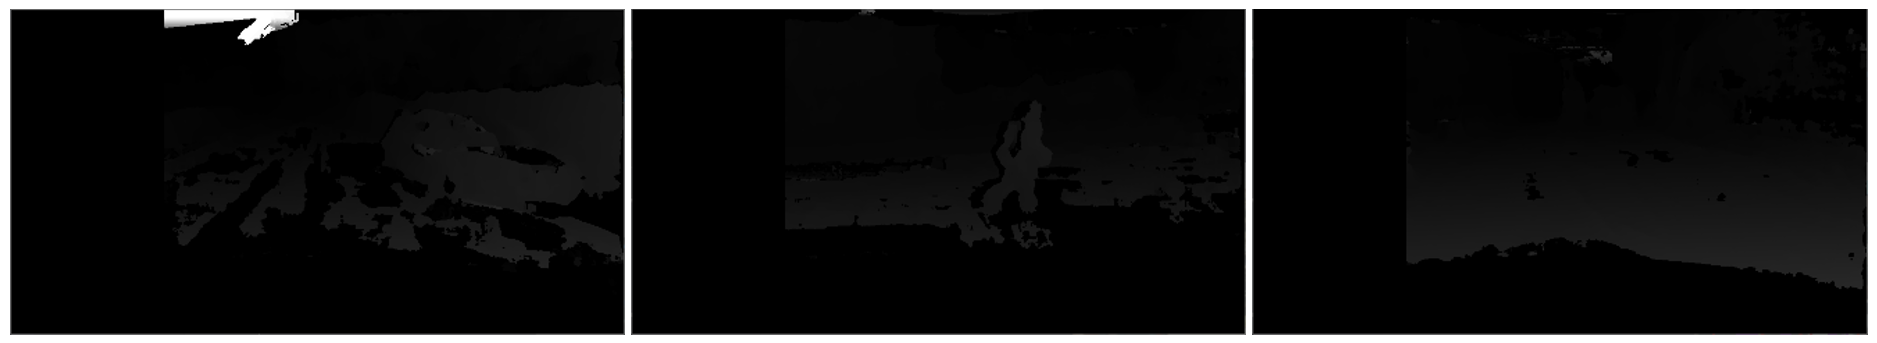
\includegraphics[width=1.0\linewidth]{"../_submission/disparity_hirschmuller.png"}
			\captionof{figure}{Disparity images calculated by the H. Hirschmuller algorithm.}
		\end{center}
	\end{minipage}

	\begin{minipage}{1.0\linewidth}
		\begin{center}
			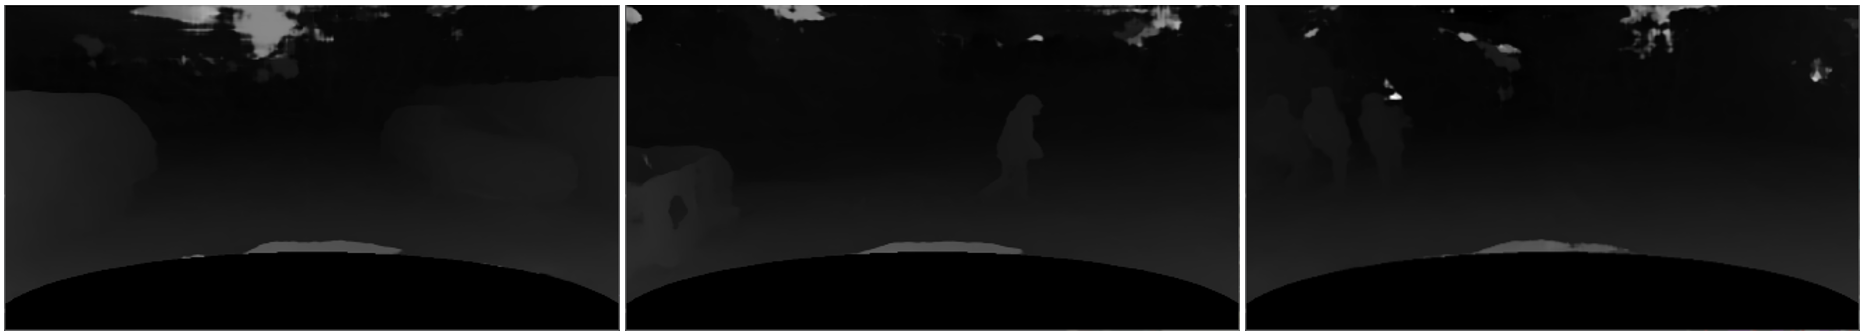
\includegraphics[width=1.0\linewidth]{"../_submission/disparity_PSMNet.png"}
			\captionof{figure}{Disparity images calculated by the Pyramid Stereo Matching Network.}
		\end{center}
	\end{minipage}


	\begin{minipage}{1.0\linewidth}
		\begin{center}
			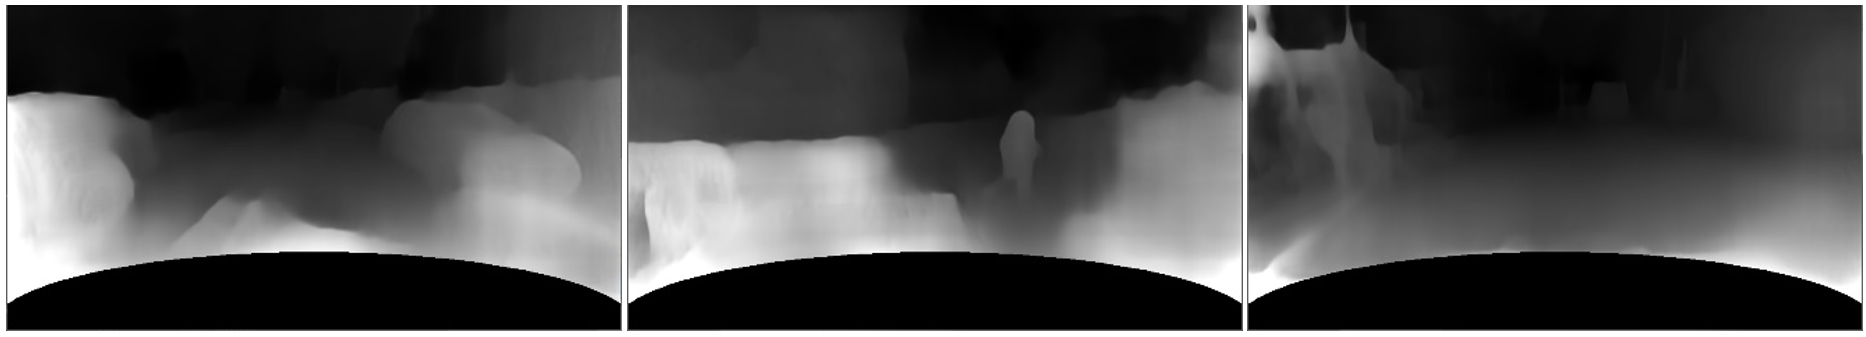
\includegraphics[width=1.0\linewidth]{"../_submission/disparity_mono-net.png"}
			\captionof{figure}{Disparity images calculated by th monocular depth network.}
		\end{center}
	\end{minipage}

	The main factors used to determine the effectiveness of the disparity solution were the ability to represent geometry on the input, the amount of noise, as-well as continuity in challenging frames.
	
	\begin{center}
		\begin{minipage}{0.33\linewidth}
		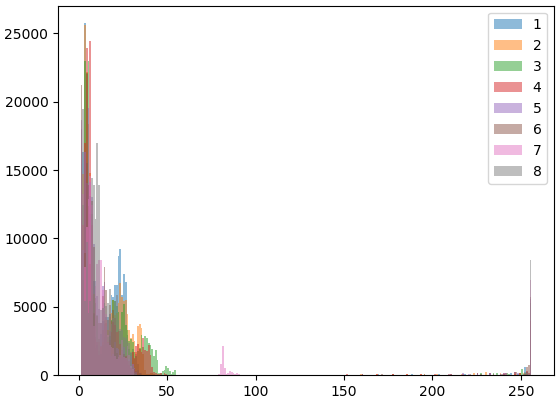
\includegraphics[width=\linewidth]{"../_submission/histogram-hirschmuller.png"}
		\begin{center}
			H. Hirschmuller
		\end{center}
		\end{minipage}%
		\hfill
		\begin{minipage}{0.33\linewidth}
		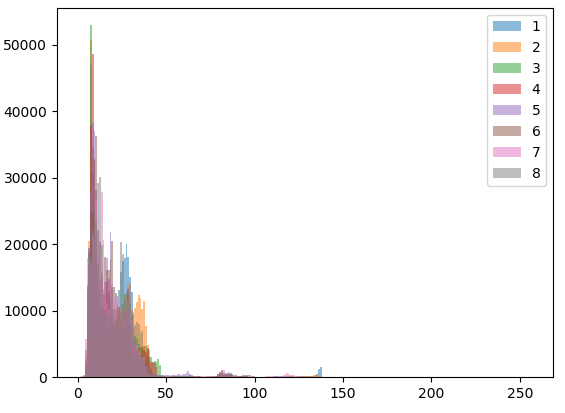
\includegraphics[width=\linewidth]{"../_submission/histogram-pyramid-matching.png"}
		\begin{center}
			PSMNet
		\end{center}
		\end{minipage}
		\hfill
		\begin{minipage}{0.33\linewidth}
			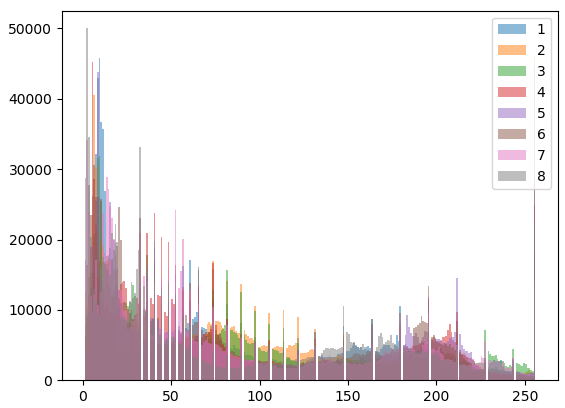
\includegraphics[width=\linewidth]{"../_submission/histogram-monocular.png"}
			\begin{center}
				MonoDepth2
			\end{center}

		\end{minipage}
		\captionof{figure}{Histograms of the above three approaches for the first 8 frames of the dataset.}
		\vspace{-1em}
	\end{center}

	As shown in figure 4, PSMNet produces the best results regarding temporal consistency and amount of error in each frame.

	\section{Estimating depth from disparity}
	
	Taking the mean of the corresponding disparity map from the bounding boxes produced by YOLO (the object detection algorithm) means that you will also include regions that are in the background of the image, thus lowering the disparity of the object unintentionally. Initially using the bounding boxes given from YOLO, a semantic segmentation approach was explored as an alternative to detect the areas of objects and what the corresponding object was. This enabled the ability to obtain the disparity from regions which could be segmented from the background, giving a more accurate disparity value. Results of the segmentation overlaid with the bounding boxes of each object are given in figure 5. The segmentation approach works well for close objects, however as objects are smaller the further away it becomes more complex to segment them properly. In most frames the segmentation map can pickup objects in the immediate vicinity of the vehicle, sometimes encountering noise in darker or blurry regions.
	
	\begin{minipage}{1.0\linewidth}
		\begin{center}
			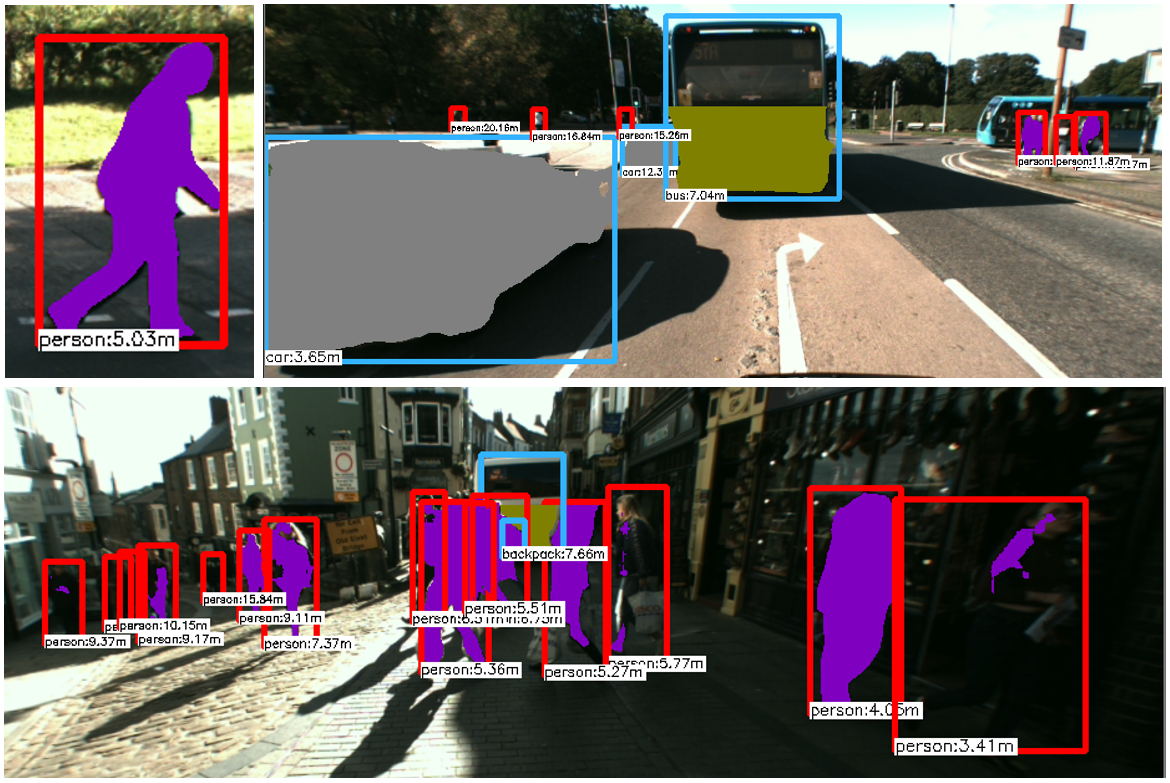
\includegraphics[width=0.67\linewidth]{"../_submission/semantic_segmentation.png"}
			\captionof{figure}{Semantic segmentation results overlaid inside the bounding boxes detected by YOLO.}
		\end{center}
	\end{minipage}
	
	
	\section{Heuristics \& Optimizations implemented}
	
	In addition to segmenting the bounding boxes, for buses, the segmentation is cropped to half its height as windows in buses can lead to discrepancies in disparity values.

	\begin{minipage}{1.0\linewidth}
	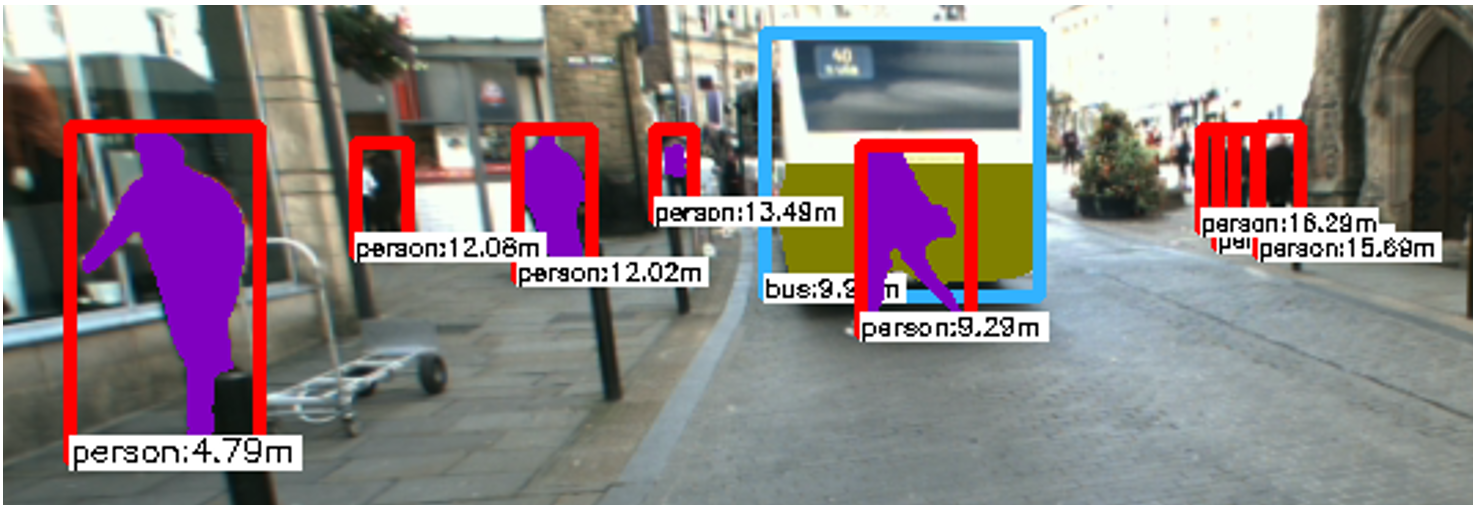
\includegraphics[width=\linewidth]{"../_submission/cut_heuristic.png"}
	\captionof{figure}{The top half of large vehicles is cut off to not use disparity calculated in regions containing windows.}
	\end{minipage}

	CLAHE (contrast limited adaptive histogram equalization) was also utilized to improve the contrast in frames where lighting was over-exposed. This led to easier recognition of objects qualitatively, and for the same test frames, YOLO was able to identify 9 more objects when using a confidence threshold of 0.55. Results of CLAHE (before and after) are given below:
	
	\begin{minipage}{1.0\linewidth}
		\begin{center}
			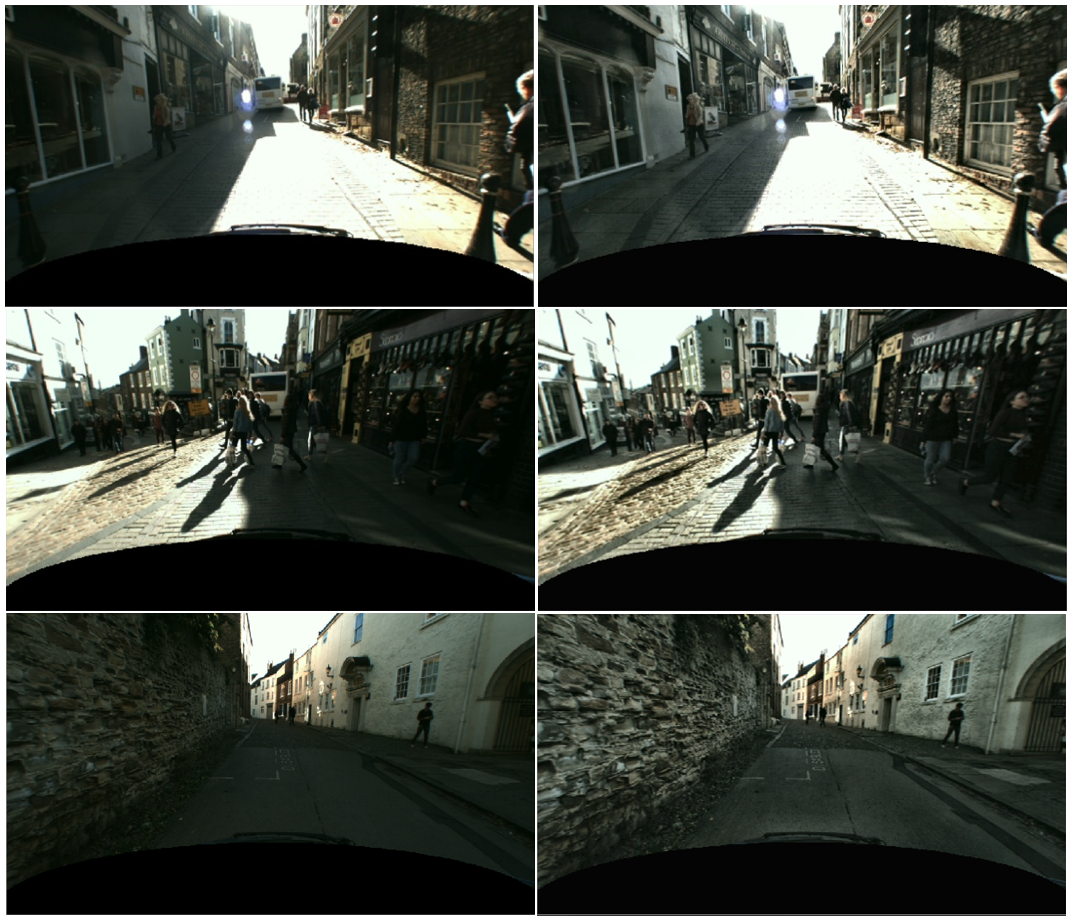
\includegraphics[width=0.76\linewidth]{"../_submission/clahe-before-and-after.png"}
			\captionof{figure}{Results of CLAHE before (left) and after (right).}
		\end{center}
	\end{minipage}
	
	When detecting objects in the scene, reflections on the bonnet of the car could cause erroneous objects to be detected. Therefore, an ellipse is sliced out of the left and right images when performing calculations on them.
	
	\begin{minipage}{1.0\linewidth}
		\begin{center}
			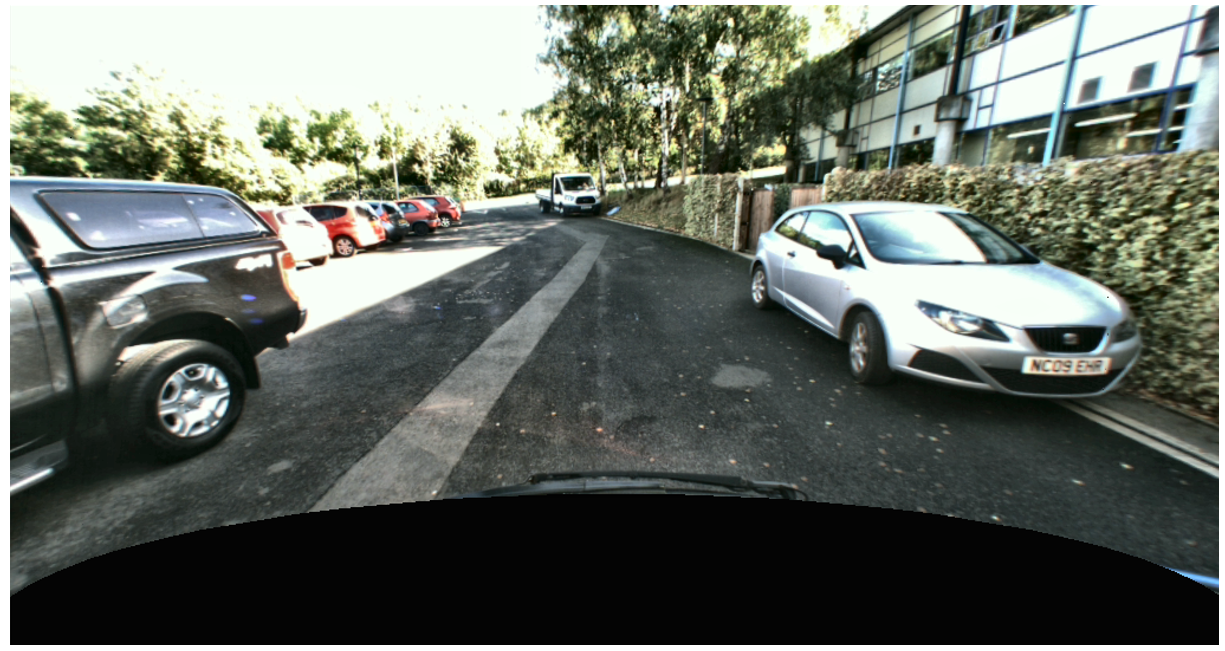
\includegraphics[width=0.76\linewidth]{"../_submission/bonnet-mask.png"}
			\captionof{figure}{The elliptical mask used on both left and right images.}
		\end{center}
	\end{minipage}

	\section{Conclusion}
	
	The per frame runtime is 2.865 seconds. The solution works well for distances up to 15m, however once objects get further away their distances are often under-predicted. For this application, accuracy of objects at larger distances isn’t as important as those that are nearby – however a possible improvement is to train using varied data and explore how scaling could lead to increased accuracy. It also handles varied lighting conditions; however, the solution may not perform well in drastically different environments such as snow due to reflections. A further extension to the current implementation would be to use Generative Adversarial Networks for reducing the effect of motion blur, e.g. DeblurGAN-v2 \cite{kupyn2019deblurganv2}.
	
	\bibliographystyle{unsrt}
	\bibliography{References}
\end{document}